En la figura \ref{fig.cto_completo} se muestra el circuito amplificador de potencia completo, donde se han identificado en línea punteada los bloques que conforman el amplificador. Se debe destacar que dicha selección de bloques es aproximada, ya que las etapas se encuentran relacionadas, es decir que comparten componentes y una etapa sin la otra podría no operar correctamente. A continuación se detallará el funcionamiento de la implementación de cada bloque, comenzando por la etapa de salida.

\begin{figure}[H]
	%\centering
	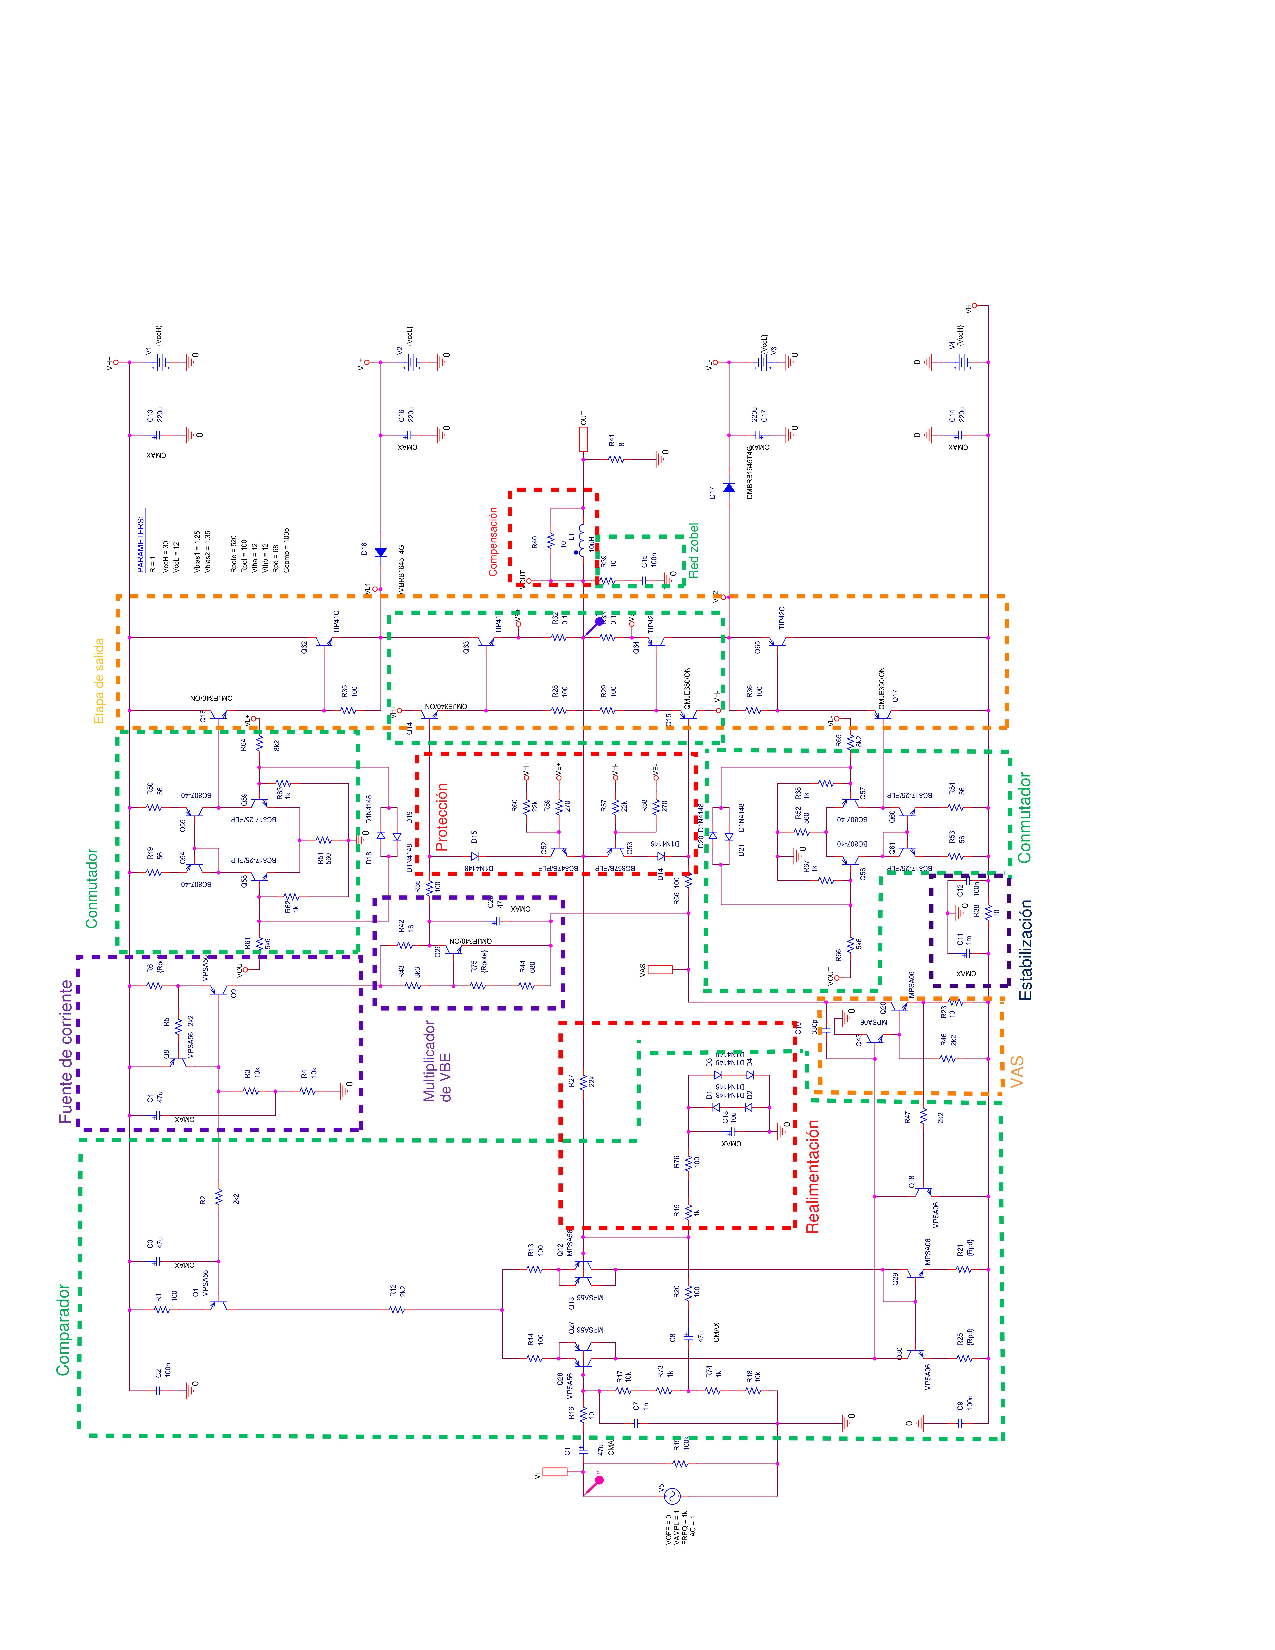
\includegraphics[scale=0.7,angle=-90]{esquema2.pdf}
	\caption{Circuito completo.}
	\label{fig.cto_completo}
\end{figure}

\pagebreak
